\section{Influence of the measurement method}
\label{sec:Method}

In the following section the difference in results performing white light reflectometry in reflection
and transmission is analyzed and discussed.

As can be seen in Figure \ref{fig:SpecRefTrans}, the measured spectra in transmission and reflection show the same tendencies with regard to the position and number of minima and maxima. The films which are coated with a higher speed of rotation show less minima and maxima in the 
observed spectral range. This is an indicator for a lower layer thickness as can be concluded from equation \ref{eq:lamdathick}, as we expect since faster spinning in coating leads to 
bigger centrifugal forces on the solution during coating. This intuitive explanation is also reflected in the experimentally determined Schubert equation. 

Furthermore we determined the mean values and the standard deviation for every measurement on the same sample. To verify wether the is a 
connection between the 


\begin{figure}[h]
    \centering
    \begin{subfigure}[b]{0.70\textwidth}
        \centering
        \input{Bilder/Auswertung/VglMessmeth/VglMessmethrefl500adn5000.tex}
        \caption{$y=x$}
        \label{fig:y equals x}
    \end{subfigure}  
    

    \begin{subfigure}[b]{0.70\textwidth}
        \centering
        \input{Bilder/Auswertung/VglMessmeth/VglMessmethtrans500adn5000.tex}   
        \caption{$y=3\sin x$} 
        \label{fig:three sin x}
    \end{subfigure}

    \caption{Spectra measured in reflectance and transmission on a thin film of PS on Glass. The films are coated with different coating speeds.}
    \label{fig:SpecRefTrans}
\end{figure}

When using the thickness output of the Nanocalc program, we observe a decrease in the coating thickness for lower concentrations of the coating solution as well as for higher rotational speeds as depicted in Figure \ref{fig:thickconcrpm}.

\begin{figure}[h]
    \centering
    \begin{subfigure}[b]{\textwidth}
        \centering
        %\resizebox{8cm}{6cm}{
        % This file was created with tikzplotlib v0.10.1.
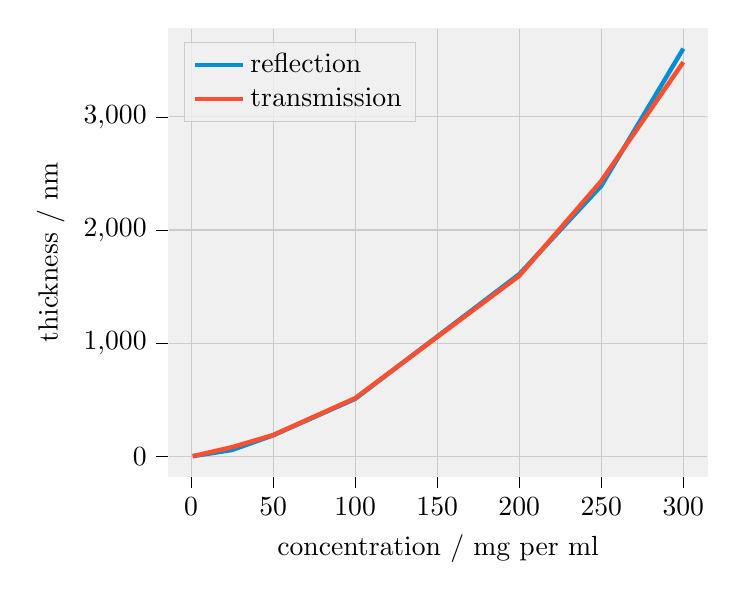
\begin{tikzpicture}

\definecolor{dodgerblue0143213}{RGB}{0,143,213}
\definecolor{lightgray203}{RGB}{203,203,203}
\definecolor{lightgray204}{RGB}{204,204,204}
\definecolor{tomato2527948}{RGB}{252,79,48}
\definecolor{whitesmoke240}{RGB}{240,240,240}

\begin{axis}[
axis background/.style={fill=whitesmoke240},
axis line style={whitesmoke240},
legend cell align={left},
legend style={
  fill opacity=0.8,
  draw opacity=1,
  text opacity=1,
  at={(0.03,0.97)},
  anchor=north west,
  draw=lightgray204,
  fill=whitesmoke240
},
tick align=outside,
tick pos=left,
x grid style={lightgray203},
xlabel={concentration / mg per ml},
xmajorgrids,
xmin=-13.95, xmax=314.95,
xtick style={color=black},
y grid style={lightgray203},
ylabel={thickness / nm},
ymajorgrids,
ymin=-180.18, ymax=3783.78,
ytick style={color=black}
]
\addplot [ultra thick, dodgerblue0143213]
table {%
1 0
25 54.8
50 184.333333333333
100 506.916666666667
200 1608.61666666667
250 2390.2
300 3603.6
};
\addlegendentry{reflection}
\addplot [ultra thick, tomato2527948]
table 
        \caption{Thickness of the film against rotation speed during coating}
        \label{fig:VglMethConcThick}
    \end{subfigure}

    \vspace{1cm}
    \begin{subfigure}[b]{\textwidth}
        \centering
        % This file was created with tikzplotlib v0.10.1.
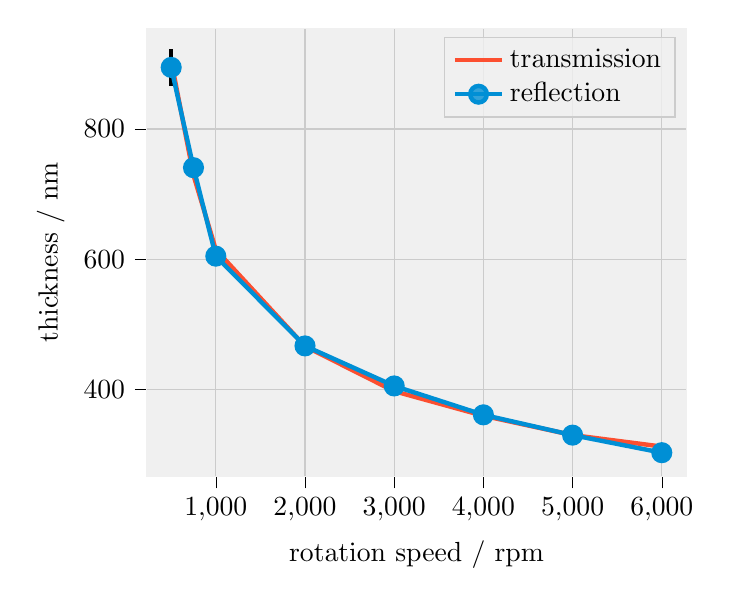
\begin{tikzpicture}

\definecolor{dodgerblue0143213}{RGB}{0,143,213}
\definecolor{lightgray203}{RGB}{203,203,203}
\definecolor{lightgray204}{RGB}{204,204,204}
\definecolor{tomato2527948}{RGB}{252,79,48}
\definecolor{whitesmoke240}{RGB}{240,240,240}

\begin{axis}[
axis background/.style={fill=whitesmoke240},
axis line style={whitesmoke240},
legend cell align={left},
legend style={fill opacity=0.8, draw opacity=1, text opacity=1, draw=lightgray204, fill=whitesmoke240},
tick align=outside,
tick pos=left,
x grid style={lightgray203},
xlabel={rotation speed / rpm},
xmajorgrids,
xmin=225, xmax=6275,
xtick style={color=black},
y grid style={lightgray203},
ylabel={thickness / nm},
ymajorgrids,
ymin=266.056164037744, ymax=954.733300161791,
ytick style={color=black}
]
\path [draw=black, ultra thick]
(axis cs:500,865.670206025666)
--(axis cs:500,923.429793974334);

\path [draw=black, ultra thick]
(axis cs:750,732.309509938563)
--(axis cs:750,748.657156728103);

\path [draw=black, ultra thick]
(axis cs:1000,599.244317659408)
--(axis cs:1000,609.955682340592);

\path [draw=black, ultra thick]
(axis cs:2000,459.903097688354)
--(axis cs:2000,473.530235644979);

\path [draw=black, ultra thick]
(axis cs:3000,398.026298881297)
--(axis cs:3000,412.407034452037);

\path [draw=black, ultra thick]
(axis cs:4000,353.366740906085)
--(axis cs:4000,368.333259093915);

\path [draw=black, ultra thick]
(axis cs:5000,314.740329019556)
--(axis cs:5000,344.593004313777);

\path [draw=black, ultra thick]
(axis cs:6000,297.359670225201)
--(axis cs:6000,308.006996441466);

\addplot [ultra thick, tomato2527948]
table {%
500 904.45
750 729.066666666667
1000 614.6
2000 466.166666666667
3000 397.166666666667
4000 359.4
5000 329.733333333333
6000 312.1
};
\addlegendentry{transmission}
\addplot [ultra thick, dodgerblue0143213, mark=*, mark size=3, mark options={solid}]
table {%
500 894.55
750 740.483333333333
1000 604.6
2000 466.716666666667
3000 405.216666666667
4000 360.85
5000 329.666666666667
6000 302.683333333333
};
\addlegendentry{reflection}
\end{axis}

\end{tikzpicture}
   
        \caption{Thickness of the film against PS concentration of the coated solution} 
        \label{fig:VglMethRotThick}
    \end{subfigure}

    \caption{Thickness output of the program \textit{NanoCalc} averaged for 6 measurement.}
    \label{fig:thickconcrpm}
\end{figure}
